\documentclass[conference]{IEEEtran}
\IEEEoverridecommandlockouts
\usepackage{cite}
\usepackage{amsmath,amssymb,amsfonts}
\usepackage{graphicx}
\usepackage{textcomp}
\usepackage{xcolor}
\usepackage{listings}
\usepackage{booktabs}
\usepackage{multirow}
\usepackage{algpseudocode}
\usepackage{algorithm}
\usepackage{url}

\def\BibTeX{{\rm B\kern-.05em{\sc i\kern-.025em b}\kern-.08em
T\kern-.1667em\lower.7ex\hbox{E}\kern-.125emX}}

\begin{document}

% -------------------------------------------------------------
\title{Optimizing LLM with FP8}

\author{
\IEEEauthorblockN{Vinh Pham Xuan}
\textit{ETC Technology Systems JSC}\\
Hanoi, Vietnam \\
phamxuanvinh023@gmail.com
\and
\IEEEauthorblockN{Khoi Nguyen Le and Vinh Nguyen Van$^\star$}
\textit{University of Engineering and Technology, }\\
Hanoi VNU\\
khoi.n.le@vnu.edu.vn,vinhnv@vnu.edu.vn
\thanks{$^\star$ Corresponding author: Vinh Nguyen Van (vinhnv@vnu.edu.vn).}
}


\maketitle

\begin{abstract}
Recent advances in low-precision arithmetic have made \textbf{FP8} \cite{micikevicius2022fp8formatsdeeplearning} a compelling alternative to FP16 and BF16 for training and inference of large language models. Rather than using a uniform FP8 format, we propose a \emph{layer-wise} specialization that assigns \textbf{E4M3} to multi-layer perceptrons (MLPs) for higher mantissa precision and \textbf{E5M2} to attention query–key paths for wider dynamic range. On \textbf{Llama-3.2-3B} and \textbf{Llama-3.1-8B} trained on 100K samples from \textbf{OpenMathInstruct-2} \cite{toshniwal2024openmath2}, our method delivers (i) \textbf{memory reduction on 3B} from \textbf{82.4 GB $\to$ 74.2 GB} (–10\%), and (ii) \textbf{training-time speedups} on both scales (\textbf{3B:} $\sim$3.6\,h $\to$ $\sim$2.1\,h; \textbf{8B:} 9.1\,h $\to$ 6.6\,h) on NVIDIA Blackwell-class GPUs. Crucially, we observe \textbf{superior numerical stability}, with \emph{loss-variance $< 0.4$} and approximately \emph{50\% lower} than a Hybrid FP8 baseline that exhibits periodic spikes $\ge 0.8$ \cite{TE2025,nvidia2024mxfp8}. These results indicate that \emph{component-aware} FP8 assignment improves stability and efficiency, with memory savings verified at 3B and time gains at both scales.
\end{abstract}

\begin{IEEEkeywords}
Large language models, FP8 precision, mixed precision training, transformer optimization, memory efficiency, computational acceleration
\end{IEEEkeywords}

\section{Introduction}

The exponential growth in large language model (LLM) parameter counts and context lengths has created unprecedented computational and memory demands. Traditional mixed-precision approaches using FP16 and BF16 formats, while effective, still impose significant memory overhead that limits model scalability and training throughput. The introduction of 8-bit floating-point (FP8) formats \cite{micikevicius2022fp8formatsdeeplearning} offers the potential to halve memory requirements while maintaining numerical stability, but current implementations face challenges in optimally leveraging the distinct characteristics of available FP8 variants.

NVIDIA\'s standardization of two FP8 formats—E4M3 (4-bit exponent, 3-bit mantissa) and E5M2 (5-bit exponent, 2-bit mantissa)—presents a fundamental trade-off between precision and dynamic range. E4M3 provides higher mantissa precision within a limited range, making it suitable for stable, dense computations, while E5M2 offers broader exponent coverage at the cost of mantissa resolution, better suited for operations with wide dynamic ranges \cite{nvidia2022fp8}.

Existing FP8 training approaches predominantly employ uniform format assignment strategies. For instance, DeepSeek-V3 \cite{deepseekv3} applies E4M3 universally across all transformer components. However, our analysis reveals that different transformer components exhibit distinct computational patterns that benefit from different FP8 formats.
This work makes the following contributions:

\begin{enumerate}
\item We present a comprehensive analysis of computational patterns across transformer components, identifying optimal FP8 format assignments based on numerical characteristics and dynamic range requirements.

\item We propose a systematic layer-wise FP8 format assignment strategy that selectively applies E4M3 to MLPs and E5M2 to attention mechanisms based on their distinct computational profiles.

\item We provide extensive experimental validation across 2 models scales (3B, 8B) and comprehensive comparison with existing FP8 approaches, demonstrating consistent improvements in memory efficiency and training throughput.

\end{enumerate}

\section{Related Work}

\subsection{Mixed-Precision Training Evolution}

Mixed-precision training has evolved from early FP16 implementations \cite{narang2017mixed} to more sophisticated approaches incorporating automatic loss scaling and gradient clipping \cite{micikevicius2018mixed}. The introduction of BF16 format addressed some numerical stability issues of FP16 by providing a wider exponent range at the cost of mantissa precision \cite{kalamkar2019study}. These approaches established the foundation for modern low-precision training strategies.

\subsection{FP8 Format Specifications and Implementations}

The IEEE 754-2019 standard introduced FP8 as a standardized low-precision format, with NVIDIA's implementation defining two specific variants optimized for deep learning workloads \cite{micikevicius2022fp8formatsdeeplearning}. The E4M3 format allocates 4 bits to the exponent and 3 bits to the mantissa, providing high precision for values within a moderate dynamic range. Conversely, E5M2 uses 5 bits for the exponent and 2 bits for the mantissa, enabling representation of values across a much wider range but with reduced precision.

Recent large-scale implementations have demonstrated FP8's viability for transformer training. DeepSeek-V3 \cite{deepseekv3} successfully trained a trillion-parameter model using uniform E4M3 formatting, achieving competitive performance with significant memory savings. However, this approach does not leverage the complementary strengths of both FP8 formats within a single model.
\subsection{Quantization-Aware Training and Format Selection}

Quantization-aware training approaches \cite{jacob2018quantization} have explored adaptive precision assignment based on layer sensitivity analysis. However, these methods primarily focus on post-training quantization or inference optimization rather than full-precision training with mixed FP8 formats. Recent work on block-wise quantization \cite{dettmers2022gpt3} demonstrates the benefits of fine-grained precision control, supporting our hypothesis that component-specific format assignment can yield significant improvements.


\section{Methodology}
\label{sec:methodology}
\subsection{Computational Pattern Analysis}

To design an effective layer-wise FP8 assignment, we analyzed the numerical behavior of major transformer components. Three main patterns emerge:

\subsubsection{MLP Stability}
Feed-forward (MLP) layers exhibit concentrated activation and gradient distributions, largely confined within moderate ranges. Since their dense matrix multiplications evolve smoothly during training, they benefit from the higher mantissa precision of \textbf{E4M3}, which better preserves small value differences.

\subsubsection{Attention Variability}
In contrast, self-attention layers display wider dynamic ranges, especially in query–key interactions:
\[
\text{Attn}(Q,K,V) = \mathrm{softmax}\!\left(\tfrac{QK^\top}{\sqrt{d_k}}\right)V.
\]
The softmax operation amplifies scale sensitivity, and attention weights often span several orders of magnitude. This motivates the use of \textbf{E5M2}, whose extended exponent range prevents overflow and underflow.

\subsubsection{Gradient Amplification}
Backpropagation through attention further increases gradient variance, particularly in query and key projections. The chain rule propagation multiplies scaling factors, producing distributions broader than those in MLP layers. Hence, stable training requires assigning formats with sufficient exponent headroom in these pathways.

\subsection{Layer-Wise Format Assignment Strategy}

Based on our analysis, we propose the following systematic assignment strategy:

\textbf{MLP Components:}
\begin{align}
\forall \ell \in \mathcal{L}_{\mathrm{MLP}}: \quad &W_{\ell}, A_{\ell}, G_{\ell} \mapsto \text{E4M3} \label{eq:mlp_assignment}
\end{align}

\textbf{Attention Components:}
\begin{align}
\forall \ell \in \mathcal{L}_{\mathrm{Attn}}: \quad &\begin{cases}
Q_{\ell}, K_{\ell} \mapsto \text{E5M2} \\
V_{\ell}, O_{\ell} \mapsto \text{E4M3} \\
G_{Q,\ell}, G_{K,\ell} \mapsto \text{E5M2} \\
G_{V,\ell}, G_{O,\ell} \mapsto \text{E4M3}
\end{cases} \label{eq:attn_assignment}
\end{align}

where $W$, $A$, and $G$ denote weights, activations, and gradients respectively, and $Q$, $K$, $V$, $O$ represent the standard attention projections.

This assignment strategy optimizes the precision-range trade-off for each component type:
- E4M3 for operations requiring high precision within moderate ranges (MLP operations, value projections)
- E5M2 for operations requiring wide dynamic range coverage (query-key interactions, attention gradients)

\subsection{Implementation Architecture}

Our implementation leverages NVIDIA's Transformer Engine to provide seamless integration with existing PyTorch workflows. Figure \ref{fig:fp8_architecture} illustrates the layer-wise FP8 format assignment within the transformer architecture, showing how E4M3 is applied to MLP components while E5M2 is selectively used for attention query-key operations.

\begin{figure}[htbp]
    \centering
    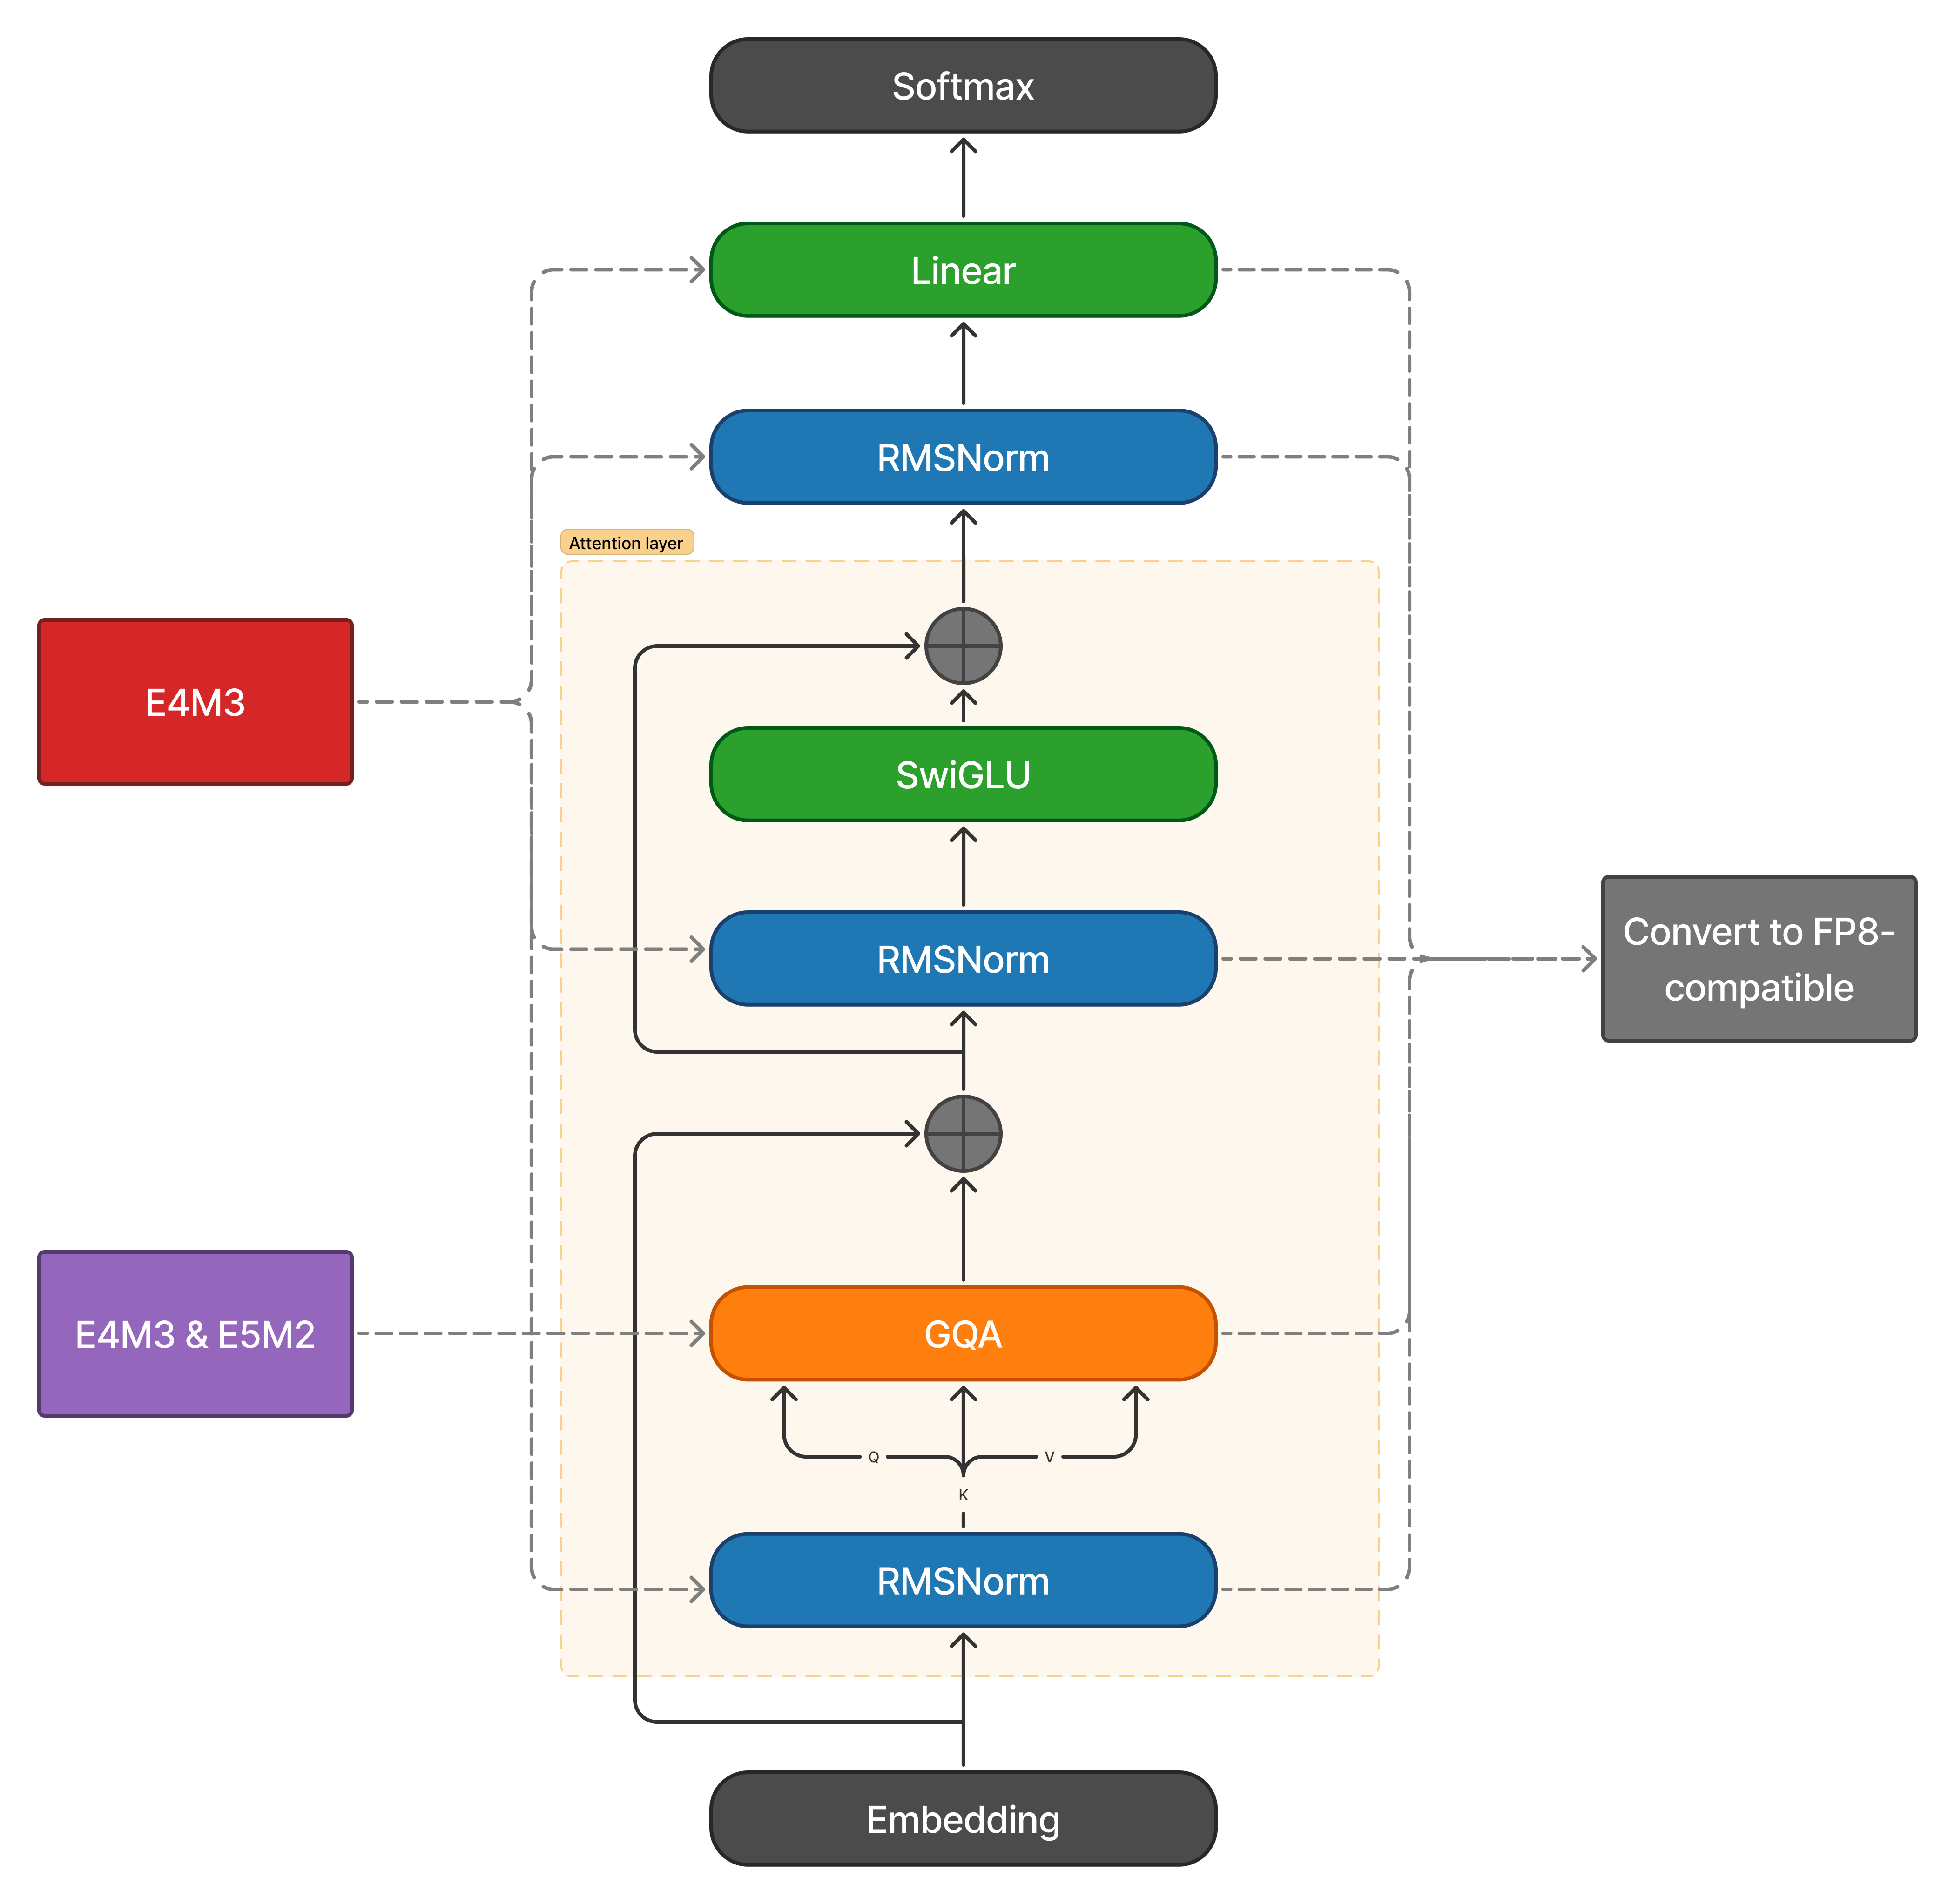
\includegraphics[width=1\columnwidth]{fp8_convert.png}
    \caption{Layer-wise FP8 format assignment architecture. The diagram shows a transformer block with selective application of E4M3 (red) for MLP layers and mixed E4M3/E5M2 (purple) for attention mechanisms. The GQA (Grouped Query Attention) module uses E5M2 for query-key operations requiring extended dynamic range, while E4M3 is applied to value projections and feed-forward networks for higher precision within stable ranges.}
    \label{fig:fp8_architecture}
\end{figure}

\noindent Algorithm~\ref{alg:layer_replacement} outlines our systematic module replacement strategy.

\begin{algorithm}[hbt!]
\caption{Layer-Wise FP8 Format Assignment}
\label{alg:layer_replacement}
\begin{algorithmic}
\Require Original model $\mathcal{M}$, FP8 configuration $\mathcal{C}$
\Ensure FP8-optimized model $\mathcal{M}_{FP8}$

\State $\mathcal{M}_{FP8} \gets \text{copy}(\mathcal{M})$

\ForAll{$\ell \in \text{transformer\_layers}(\mathcal{M}_{FP8})$}
    \State // MLP format assignment (E4M3)
    \State $\ell.\text{mlp}.fc1 \gets \text{FP8Linear}(\ell.\text{mlp}.fc1, \text{E4M3})$
    \State $\ell.\text{mlp}.fc2 \gets \text{FP8Linear}(\ell.\text{mlp}.fc2, \text{E4M3})$
    
    \State // Attention format assignment (mixed)
    \State $\ell.\text{attn}.q\_proj \gets \text{FP8Linear}(\ell.\text{attn}.q\_proj, \text{E5M2})$
    \State $\ell.\text{attn}.k\_proj \gets \text{FP8Linear}(\ell.\text{attn}.k\_proj, \text{E5M2})$
    \State $\ell.\text{attn}.v\_proj \gets \text{FP8Linear}(\ell.\text{attn}.v\_proj, \text{E4M3})$
    \State $\ell.\text{attn}.o\_proj \gets \text{FP8Linear}(\ell.\text{attn}.o\_proj, \text{E4M3})$
\EndFor

\State \Return $\mathcal{M}_{FP8}$
\end{algorithmic}
\end{algorithm}

\subsection{Training Loop Integration}

Algorithm \ref{alg:fp8_training} presents our enhanced training procedure that incorporates dynamic format selection and optimized scaling strategies.

\begin{algorithm}[hbt!]
\caption{FP8 Training Step with Layer-Wise Format Assignment}
\label{alg:fp8_training}
\begin{algorithmic}
\Require Mini-batch $\mathcal{B}$, parameters $\Theta_t$, FP8 config $\mathcal{C}$
\Ensure Updated parameters $\Theta_{t+1}$, loss $\mathcal{L}$

\State \textbf{Forward Pass}
\ForAll{$\ell \in \mathcal{L}_{\mathrm{MLP}}$}
  \State $A_\ell^{\text{E4M3}} \gets \text{quantize}(A_{\ell}, \text{E4M3}, \mathcal{C})$
  \State $W_\ell^{\text{E4M3}} \gets \text{quantize}(W_{\ell}, \text{E4M3}, \mathcal{C})$
  \State $Z_\ell \gets \text{GEMM}(A_\ell^{\text{E4M3}}, W_\ell^{\text{E4M3}})$
\EndFor

\ForAll{$\ell \in \mathcal{L}_{\mathrm{Attn}}$}
  \State $Q_\ell^{\text{E5M2}} \gets \text{quantize}(Q_{\ell}, \text{E5M2}, \mathcal{C})$
  \State $K_\ell^{\text{E5M2}} \gets \text{quantize}(K_{\ell}, \text{E5M2}, \mathcal{C})$
  \State $V_\ell^{\text{E4M3}} \gets \text{quantize}(V_{\ell}, \text{E4M3}, \mathcal{C})$
  \State $\text{Attn}_\ell \gets \text{ScaledDotProduct}(Q_\ell^{\text{E5M2}}, K_\ell^{\text{E5M2}}, V_\ell^{\text{E4M3}})$
\EndFor

\State $\mathcal{L} \gets \text{ComputeLoss}(\text{model\_output}, \text{targets})$

\State \textbf{Backward Pass}
\State Apply format-specific gradient quantization according to Eq.~\ref{eq:mlp_assignment}-\ref{eq:attn_assignment}

\State \textbf{Parameter Update}
\State Update parameters with FP32 accumulation
\State \Return $\Theta_{t+1}, \mathcal{L}$
\end{algorithmic}
\end{algorithm}


\section{Experimental Setup}

\subsection{Model Architectures and Scales}
\textbf{Llama-3.2-3B} \cite{meta2024llama3.2} and \textbf{Llama-3.1-8B} \cite{meta2024llama3.1}.

\subsection{Dataset and Training Configuration}
\textbf{Dataset:} OpenMathInstruct-2 \cite{toshniwal2024openmath2}, 100K instruction–response pairs.\\
\textbf{Schedule:} 3 epochs, sequence length 512, AdamW, grad accumulation 4.
\begin{table}[htbp]
\centering
\caption{Training Configuration Across Model Scales}
\begin{tabular}{@{}lcc@{}}
\toprule
\textbf{Configuration} & \textbf{Llama-3.2-3B} & \textbf{Llama-3.1-8B} \\
\midrule
Batch Size (BF16) & 24 & 6 \\
Batch Size (FP8) & 24 & 6 \\
Sequence Length & 512 & 512 \\
Learning Rate & 1e-5 & 1e-5 \\
Epochs & 3 & 3 \\
Training Samples & 100K & 100K \\
Optimizer & AdamW & AdamW \\
Gradient Accumulation & 4 & 4 \\
\bottomrule
\end{tabular}
\label{tab:training_config}
\end{table}

\subsection{Baseline Comparisons}
\begin{enumerate}
\item \textbf{BF16}: standard mixed precision baseline \cite{kalamkar2019study}
\item \textbf{Hybrid FP8}: NVIDIA Hybrid (delayed scaling) using E4M3/E5M2 across layers \cite{nvidia2024mxfp8,TE2025}
\item \textbf{Ours}: layer-wise FP8 (E5M2 for Q/K; E4M3 for MLP/V/O)
\end{enumerate}

\subsection{Hardware and Software Environment}
NVIDIA Blackwell-class GPUs (96\,GB), CUDA 12.9, PyTorch 2.7+, Transformer Engine 2.5.0, Accelerate 0.34+.

\subsection{Evaluation Metrics}
Training efficiency (time, tokens/s, VRAM), model quality (perplexity, reasoning), numerical stability (loss variance), and resource utilization.

\section{Results and Analysis}

\subsection{Memory Efficiency and Training Time}
\begin{figure}[htbp]
    \centering
    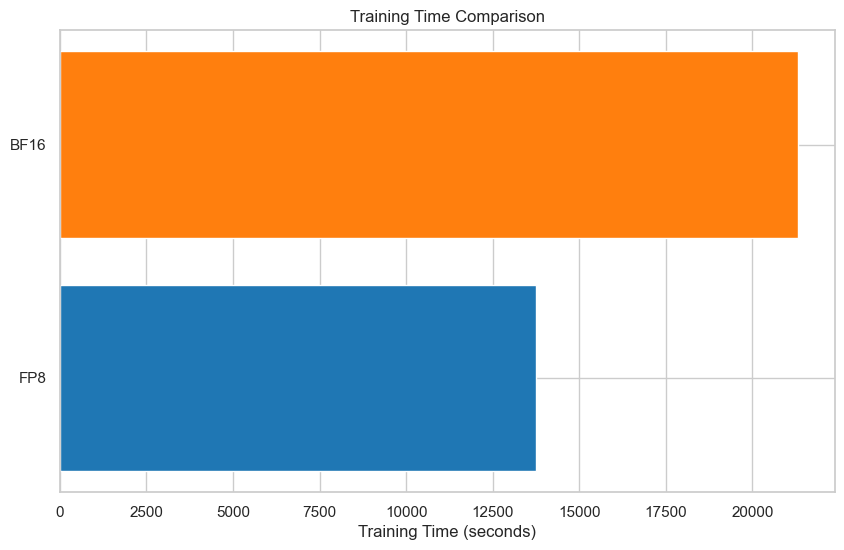
\includegraphics[width=1\columnwidth]{training_time.png}
    \caption{Relative training time comparison. In our runs FP8 configurations achieve \textbf{1.3–1.7$\times$} speedups over BF16 depending on scale.}
    \label{fig:training_time}
\end{figure}

\begin{table}[htbp]
\centering
\caption{Memory Utilization and Training Time}
\begin{tabular}{@{}lcccc@{}}
\toprule
\textbf{Model} & \textbf{Precision} & \textbf{VRAM (GB)} & \textbf{Time} \\
\midrule
\multirow{3}{*}{Llama-3.2-3B} & BF16 & 82.4 & $\sim$3.6 h \\
 & Hybrid & 74.2 & $\sim$2.2 h \\
 & FP8 (Ours) & \textbf{74.2} & \textbf{$\sim$2.1 h} \\
\midrule
\multirow{3}{*}{Llama-3.1-8B} & BF16 & \textbf{80.0} & $\sim$9.1 h \\
 & Hybrid & 88.0 & $\sim$7.6 h \\
 & FP8 (Ours) & 88.3 & \textbf{$\sim$6.6 h} \\
\bottomrule
\end{tabular}
\label{tab:memory_scaling}
\end{table}

\noindent\textbf{Findings.} FP8 reduces memory by \textbf{10\%} on \textbf{3B} (82.4$\to$74.2\,GB) and improves training time from $\sim$3.6\,h (BF16) to $\sim$2.1\,h (ours), closely matching the Hybrid FP8 baseline ($\sim$2.2\,h). For \textbf{8B}, our method achieves \textbf{6.6\,h} vs \textbf{7.6\,h} (Hybrid) and \textbf{9.1\,h} (BF16). In our setup, \textbf{8B} FP8 configurations show \emph{higher allocated VRAM} ($\sim$88\,GB) than BF16 ($\sim$80\,GB), likely due to workspace and scaling-metadata overheads; thus memory savings are \textbf{confirmed at 3B} and \emph{not universal across scales} in our current implementation.

\subsection{Convergence and Model Quality}
\begin{figure}[htbp]
    \centering
    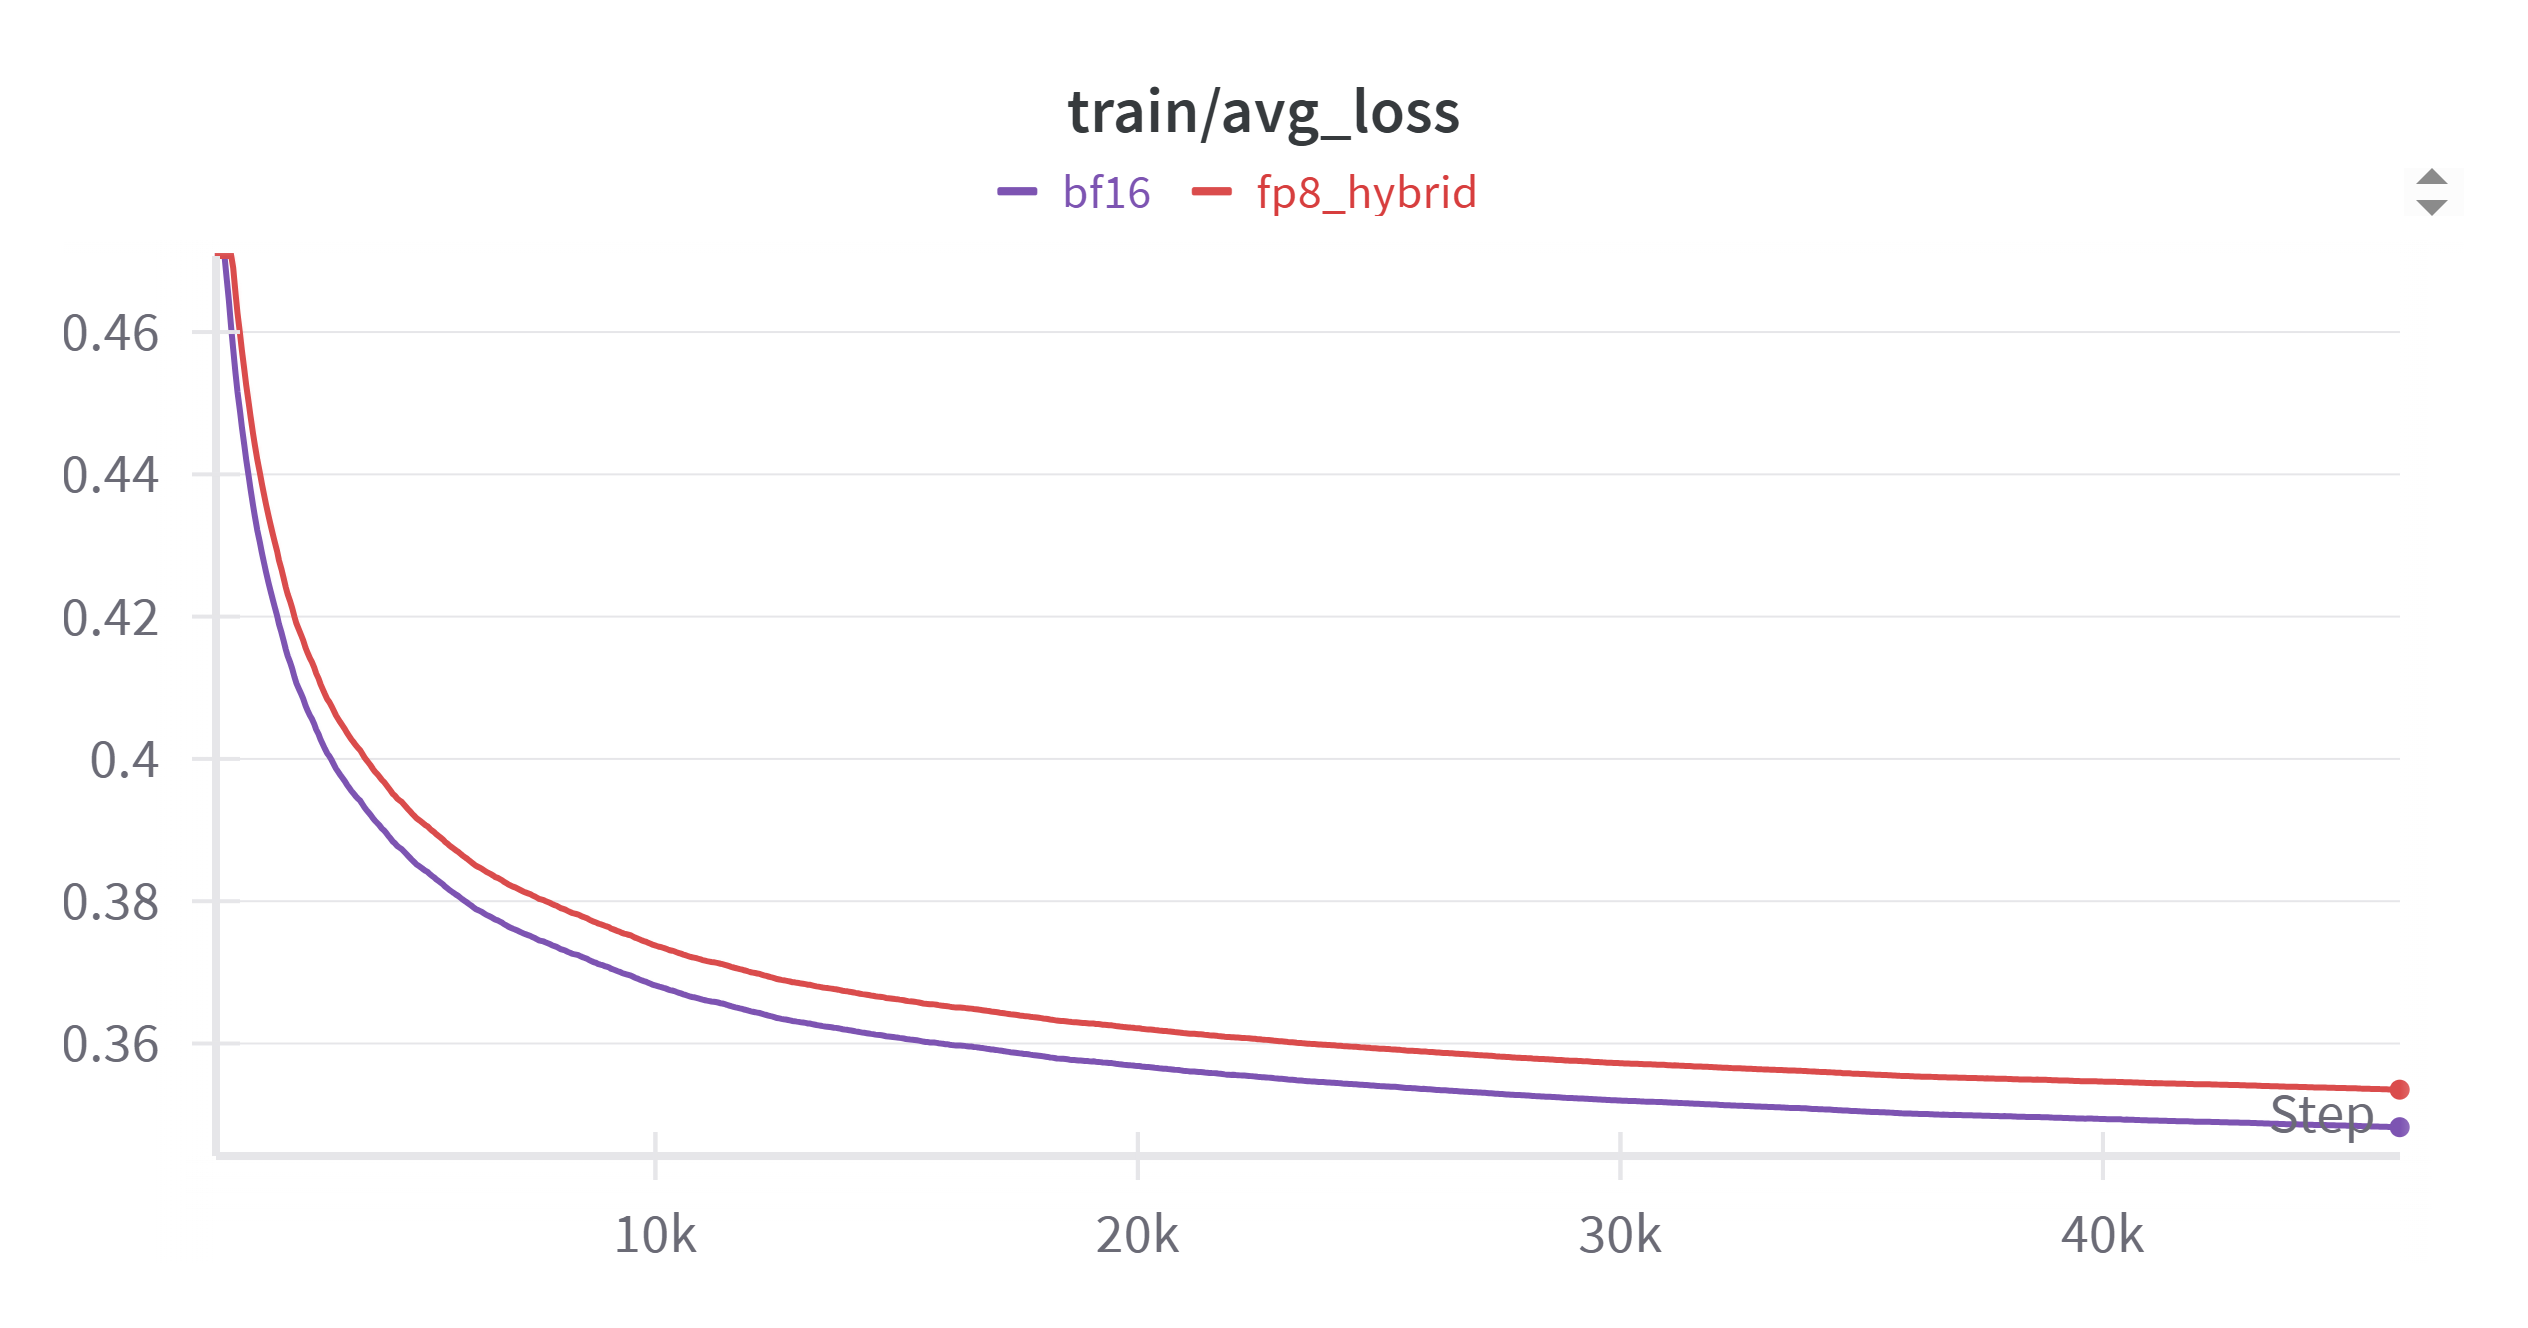
\includegraphics[width=1\columnwidth]{avg_loss.png}
    \caption{Average training loss for BF16 vs FP8 Hybrid/Ours. Final loss values are comparable; our layer-wise FP8 shows smoother dynamics.}
    \label{fig:training_loss}
\end{figure}

Both methods converge from $\sim$0.47 to $<0.36$; our layer-wise FP8 maintains lower variance and smoother dynamics.

\subsection{Numerical Stability Analysis}
\begin{figure}[htbp]
    \centering
    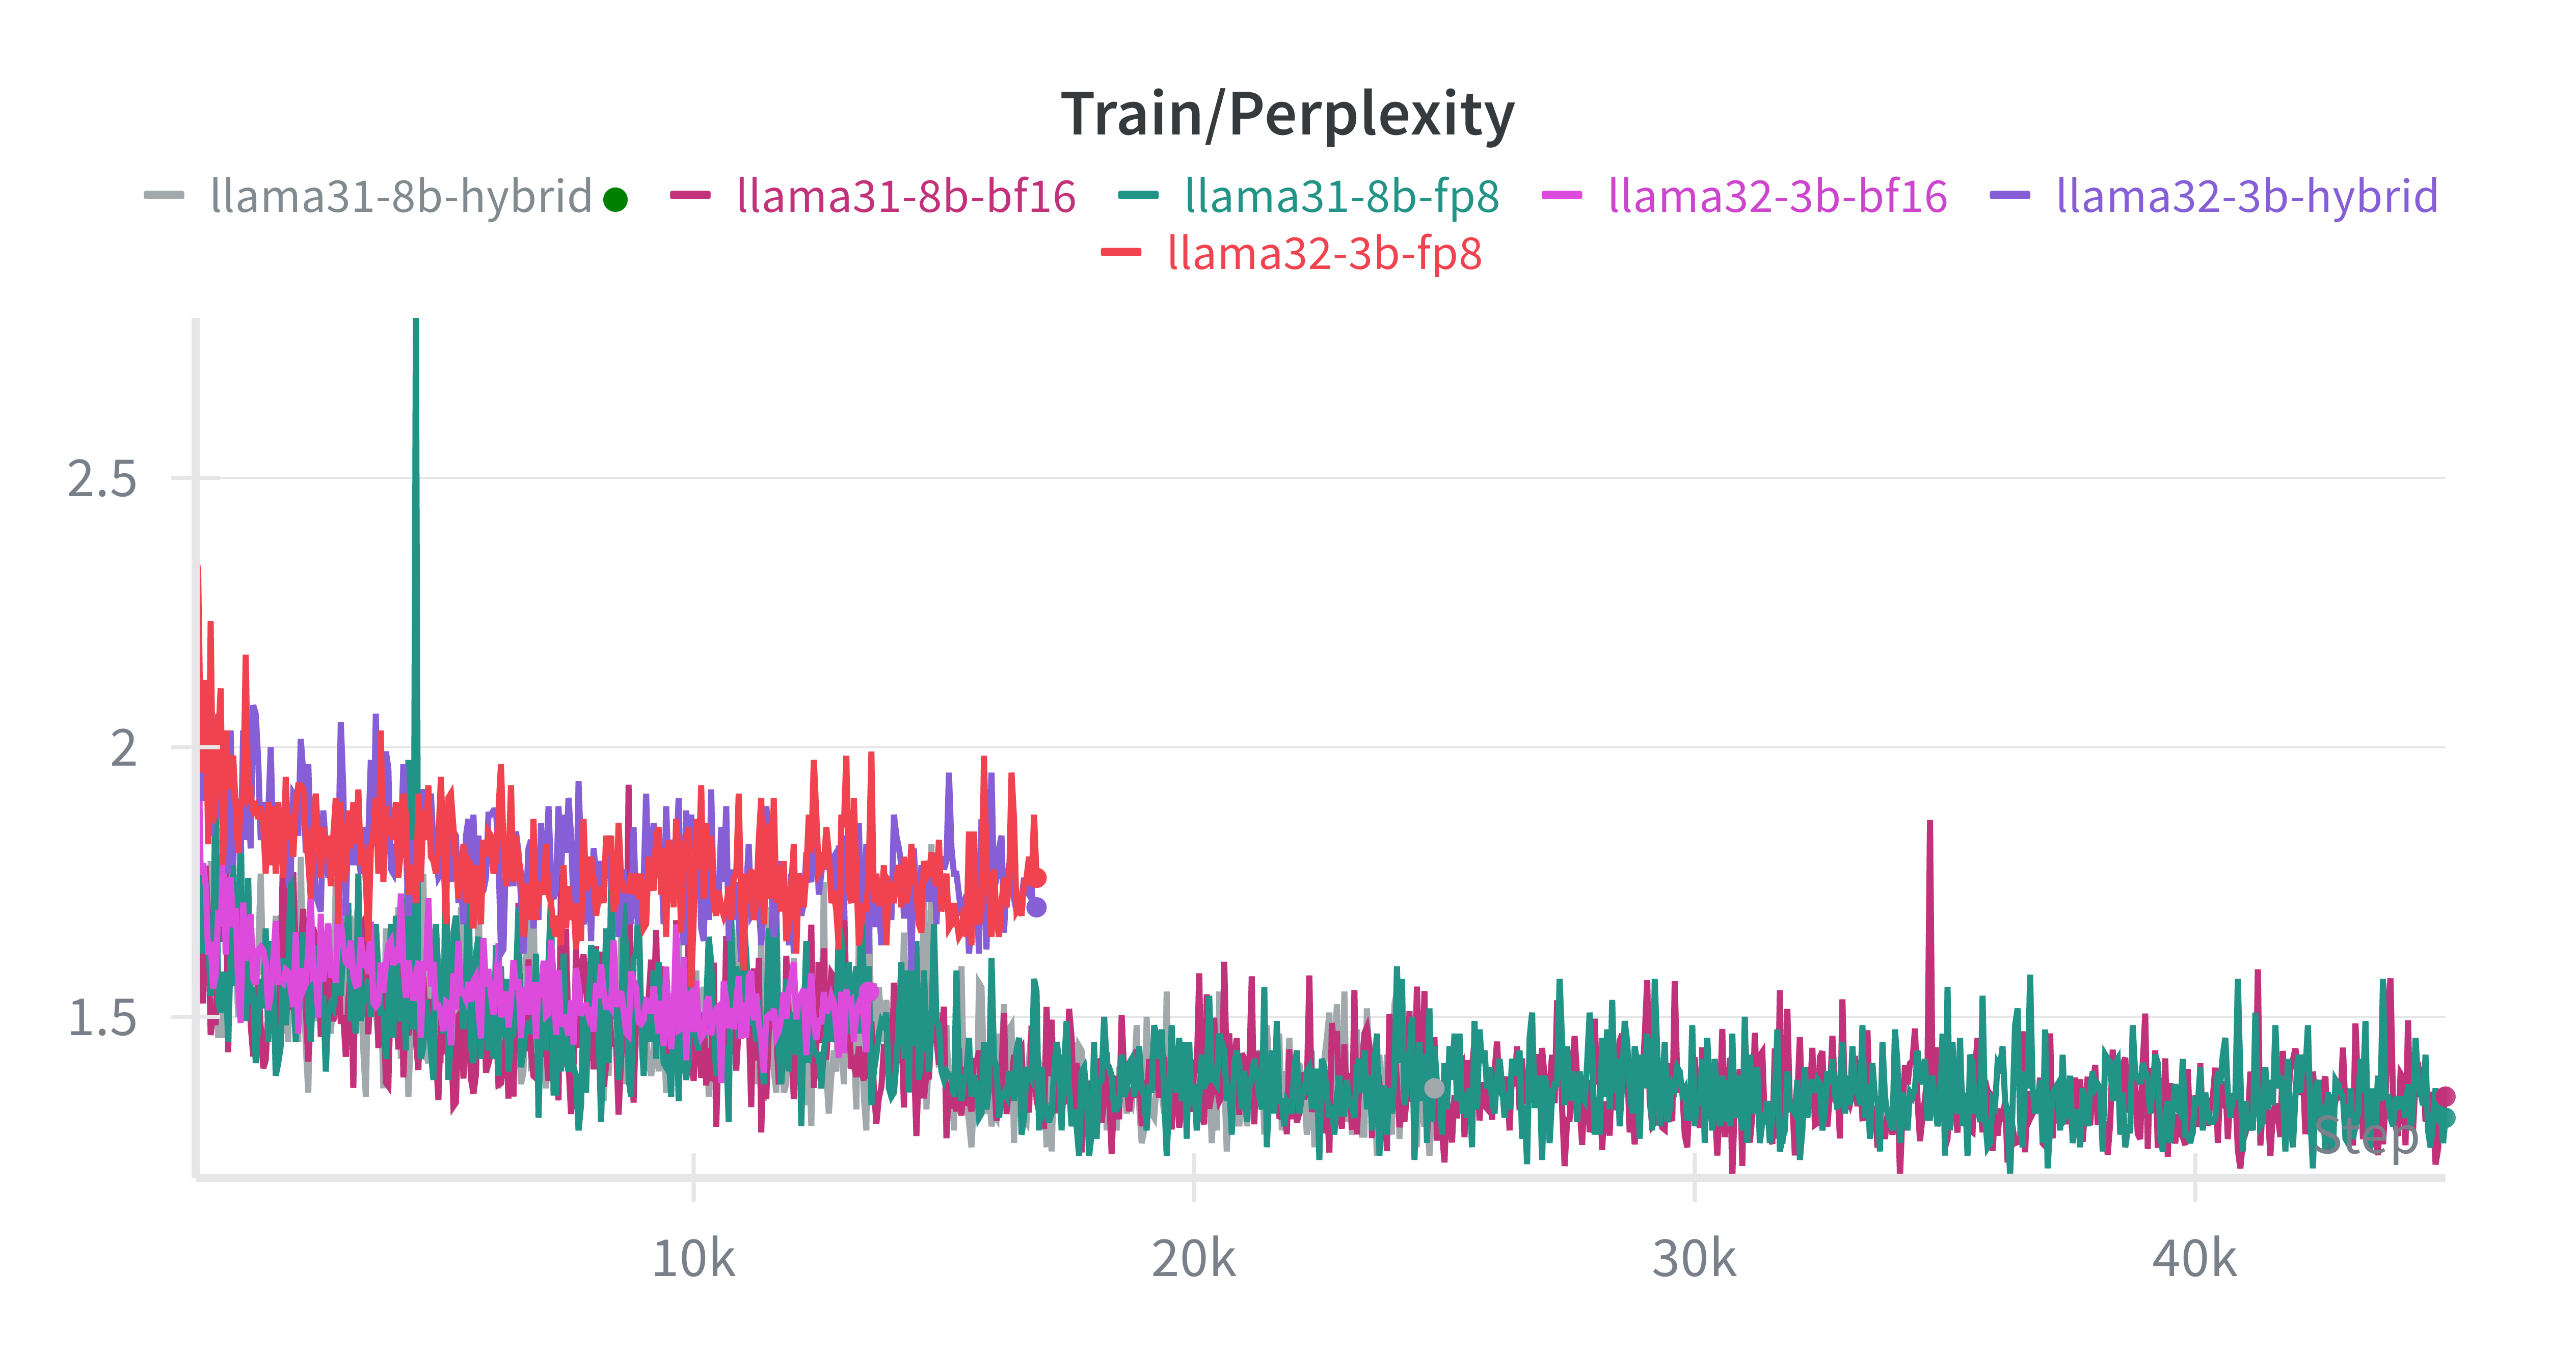
\includegraphics[width=1\columnwidth]{train_perplexity.png}
    \caption{Training perplexity across scales and precisions. Our layer-wise FP8 maintains perplexity in the 1.30–1.32 range with stable behavior.}
    \label{fig:perplexity_analysis}
\end{figure}

\begin{figure}[htbp]
    \centering
    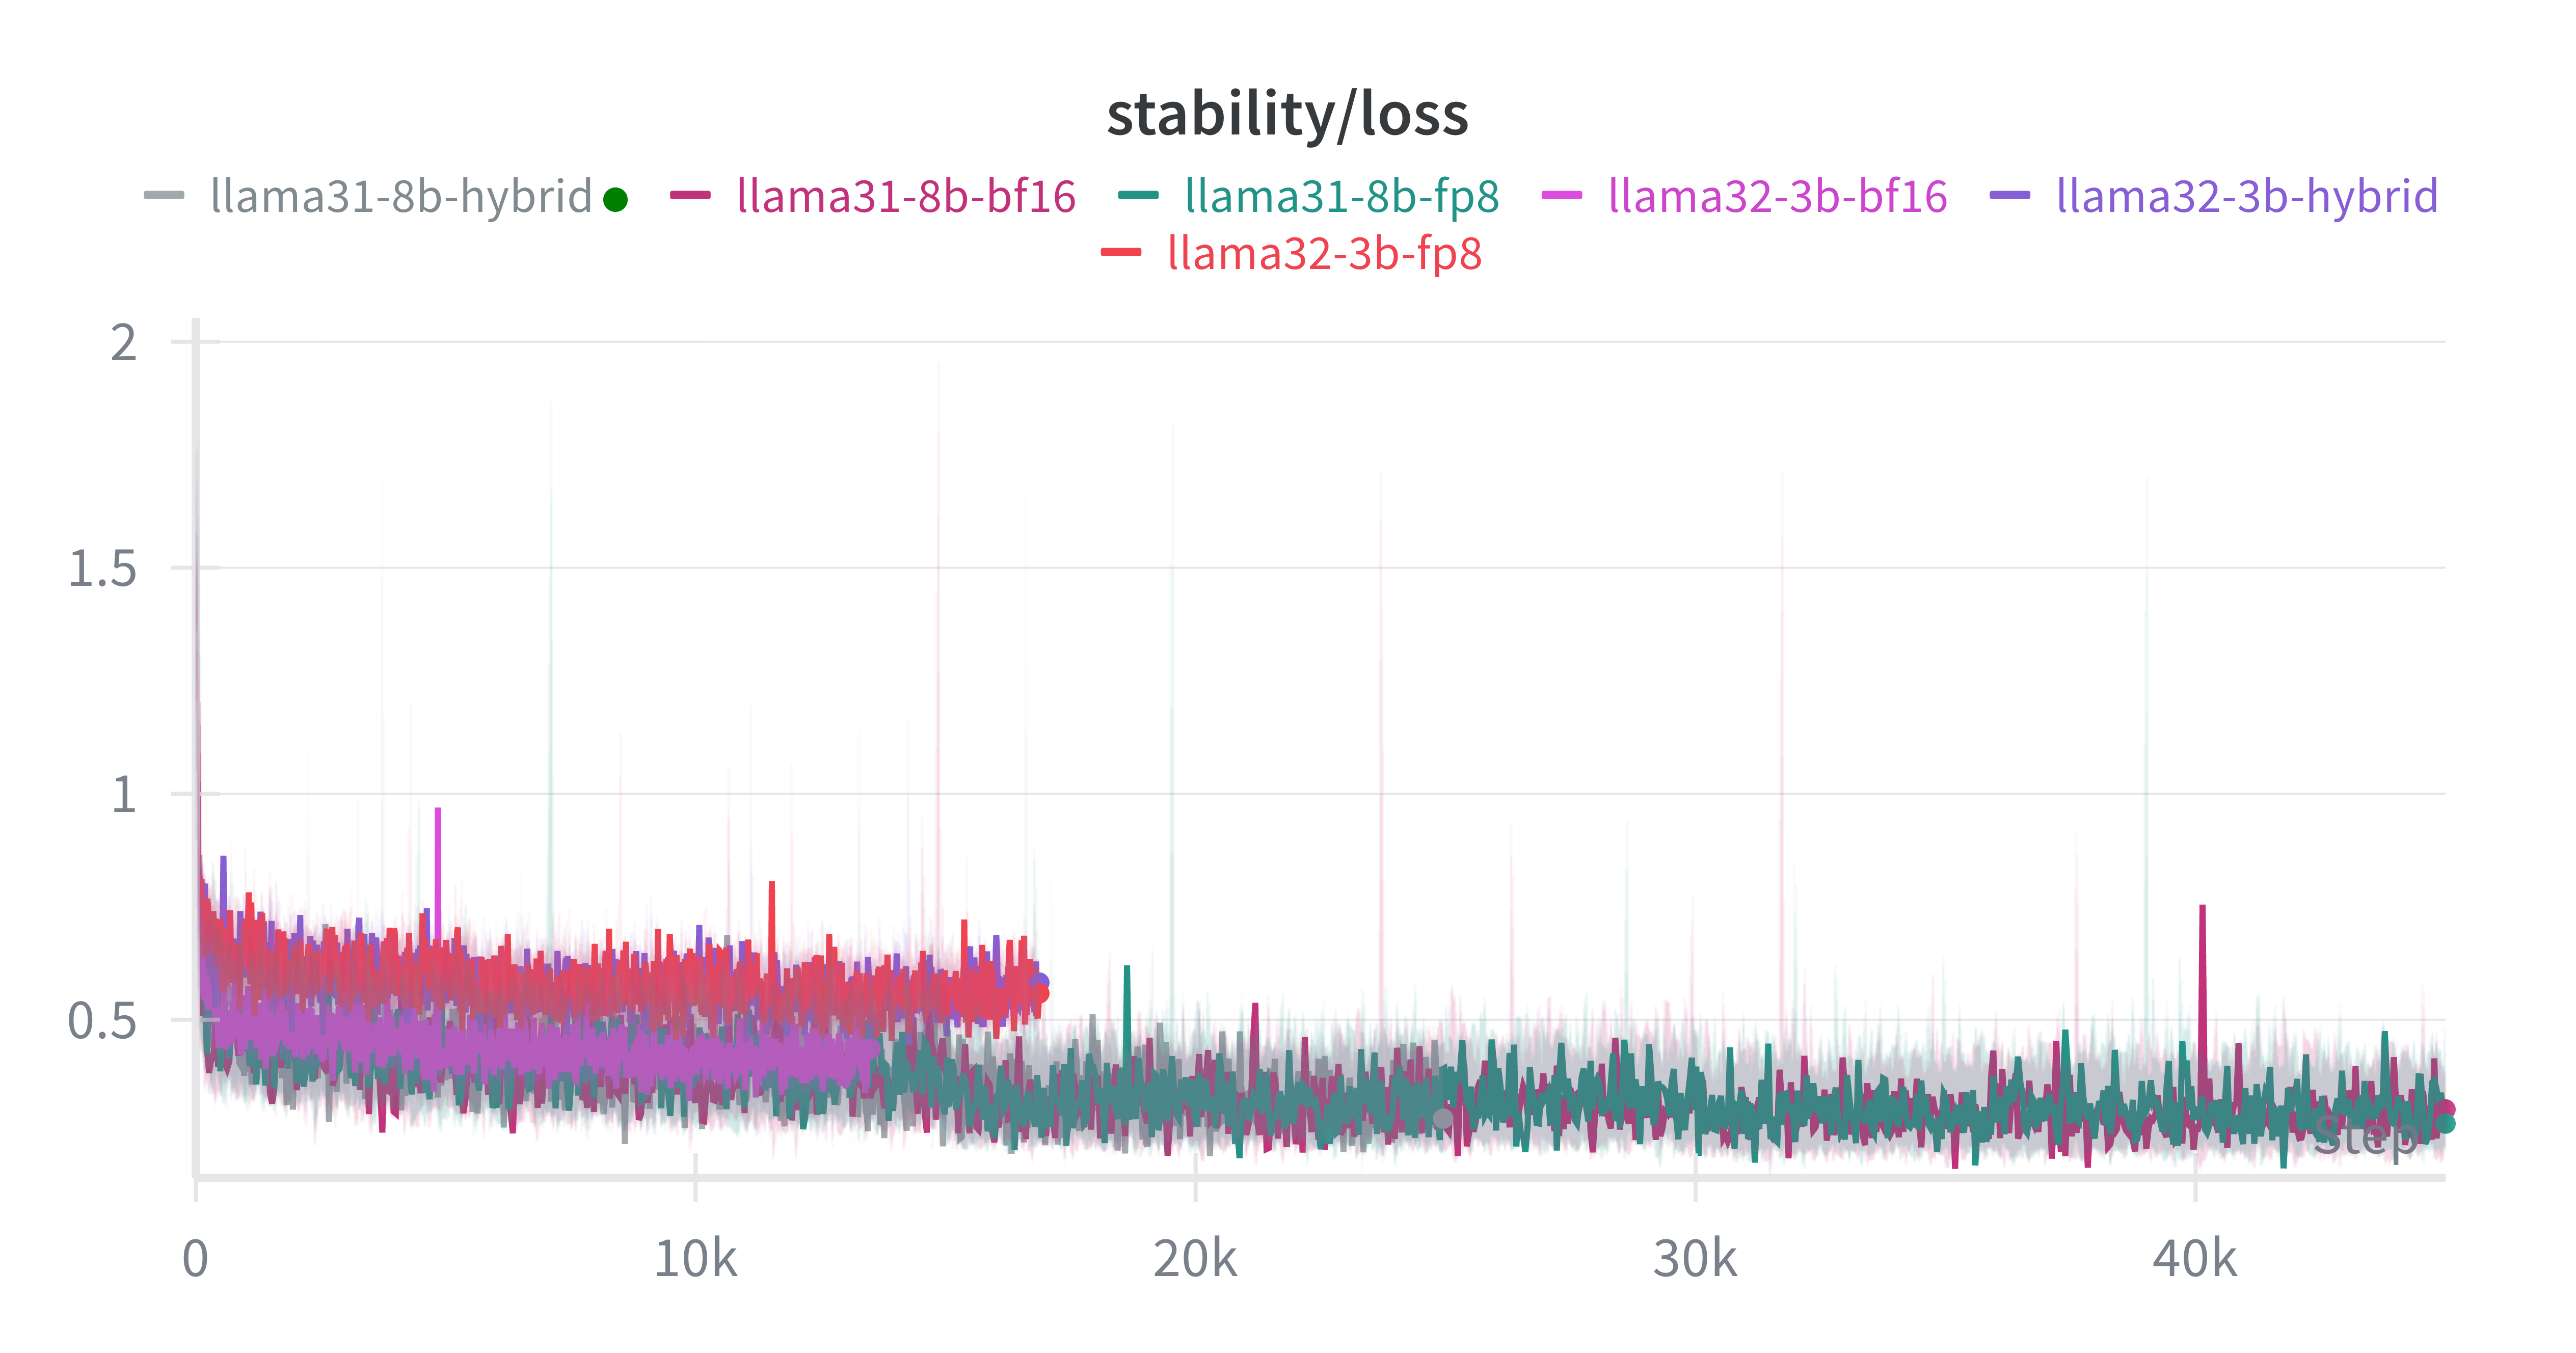
\includegraphics[width=1\columnwidth]{numeric_stability.png}
    \caption{Loss variance over steps. Our layer-wise FP8 (gray) stays \textbf{$<0.4$}; Hybrid FP8 shows periodic spikes reaching $\ge 0.8$.}
    \label{fig:stability_analysis}
\end{figure}

Selective use of E5M2 for high-dynamic-range paths (Q/K) and E4M3 elsewhere yields \textbf{lower variance} (about \textbf{50\%} less than Hybrid), improving stability.

\section{Discussion}

\subsection{Performance Analysis}
\textbf{Memory--Speed Trade-off.} At \textbf{3B}, FP8 reduces memory by 10\% and shortens training time (\~2.1\,h vs \~3.6\,h). At \textbf{8B}, we observe \emph{time speedups} but \emph{no memory reduction} in our implementation (likely due to additional workspaces/metadata).

\textbf{Method Comparison.} Layer-wise FP8 achieves \textbf{superior stability} (variance $<0.4$) compared to Hybrid FP8 (spikes $\ge 0.8$) \cite{nvidia2024mxfp8,TE2025}.

\textbf{Practical Implications.} Memory savings at \textbf{3B} enable tighter resource budgets; time gains appear at both scales, larger at \textbf{8B}.

\subsection{Limitations and Future Work}
Evaluation is limited to two Llama scales; generalization to larger models (e.g., 70B), other architectures (MoE, sparse), dynamic per-layer or per-token formats, and tighter hardware co-design are promising directions.

\section{Conclusion}

We presented a \textbf{layer-wise FP8} assignment strategy—E5M2 for attention query–key and E4M3 for MLP/value/output projections—motivated by component-specific numerical behavior. On \textbf{Llama-3.2-3B} and \textbf{Llama-3.1-8B} with \textbf{OpenMathInstruct-2} \cite{toshniwal2024openmath2}, we observed: (1) \textbf{3B memory savings} (82.4$\to$74.2\,GB, –10\%), and (2) \textbf{training-time speedups} at both scales (3B: $\sim$2.1\,h vs $\sim$3.6\,h; 8B: 6.6\,h vs 9.1\,h). Our method also delivers \textbf{50\% lower loss variance} than a Hybrid FP8 baseline \cite{nvidia2024mxfp8,TE2025}. While memory reductions were \emph{not universal} at 8B in our setup, the combination of stability and time gains highlights component-aware FP8 as a practical path to efficient LLM training.

\section*{Acknowledgments}
We thank the open-source community for tools/datasets, NVIDIA for Transformer Engine and hardware documentation, and the research community for feedback.

\begin{thebibliography}{40}

\bibitem{micikevicius2022fp8formatsdeeplearning}
P.~Micikevicius, D.~Stosic, N.~Burgess, M.~Cornea, P.~Dubey, R.~Grisenthwaite, 
S.~Ha, A.~Heinecke, P.~Judd, J.~Kamalu, N.~Mellempudi, S.~Oberman, 
M.~Shoeybi, M.~Siu, and H.~Wu, 
``FP8 Formats for Deep Learning,'' 
\emph{arXiv preprint} arXiv:2209.05433, 2022.

\bibitem{nvidia2022fp8}
NVIDIA Corporation,
``FP8 formats for deep learning,''
NVIDIA Technical Report, 2022.

\bibitem{deepseekv3}
DeepSeek-AI,
``DeepSeek-V3: A Strong, Economical, and Efficient Mixture-of-Experts Language Model,''
\emph{arXiv preprint arXiv:2412.19437}, 2024.

\bibitem{nvidia2024mxfp8}
NVIDIA Corporation,
``MXFP8: Advanced Mixed-Precision Training for Transformer Models,''
NVIDIA Technical Report, 2024.

\bibitem{narang2017mixed}
S.~Narang, G.~Diamos, S.~Sengupta, and E.~Elsen,
``Mixed precision training,''
in \emph{International Conference on Learning Representations (ICLR)}, 2017.

\bibitem{micikevicius2018mixed}
P.~Micikevicius, S.~Narang, J.~Alben, G.~Diamos, E.~Elsen, D.~Garcia, B.~Ginsburg, M.~Houston, O.~Kuchaiev, G.~Venkatesh, and H.~Wu,
``Mixed precision training,''
in \emph{International Conference on Learning Representations}, 2018.

\bibitem{kalamkar2019study}
D.~Kalamkar, D.~Mudigere, N.~Mellempudi, D.~Das, K.~Banerjee, S.~Avancha, et~al.,
``A Study of BFloat16 for Deep Learning Training,''
\emph{arXiv preprint arXiv:1905.12322}, 2019.

\bibitem{jacob2018quantization}
B.~Jacob, S.~Kligys, B.~Chen, M.~Zhu, M.~Tang, A.~Howard, H.~Adam, and D.~Kalenichenko,
``Quantization and Training of Neural Networks for Efficient Integer-Arithmetic-Only Inference,''
in \emph{CVPR}, 2018, pp.~2704--2713.

\bibitem{dettmers2022gpt3}
T.~Dettmers, M.~Lewis, Y.~Belkada, and L.~Zettlemoyer,
``GPT3.int8(): 8-bit Matrix Multiplication for Transformers at Scale,''
in \emph{NeurIPS}, vol.~35, 2022, pp.~30318--30332.

\bibitem{TE2025}
NVIDIA,
``Transformer Engine: Accelerating Transformer Models with FP8 Precision,''
NVIDIA Deep Learning Documentation, 2025.

\bibitem{meta2024llama3.2}
Meta AI, 
``Llama 3.2: Collection of foundation models for global languages and vision,'' 
Meta AI Blog, September 25, 2024.

\bibitem{meta2024llama3.1}
Meta AI,
``Llama 3.1: Our most capable models to date,''
Meta AI Blog, July 23, 2024.

\bibitem{qwen2024}
Qwen Team,
``Qwen2.5: A Party of Foundation Models,''
Qwen Technical Report, 2024.

\bibitem{toshniwal2024openmath2}
S.~Toshniwal, W.~Du, I.~Moshkov, B.~Kisacanin, A.~Ayrapetyan, and I.~Gitman, 
``OpenMathInstruct-2: Accelerating AI for Math with Massive Open-Source Instruction Data,'' 
\emph{arXiv preprint arXiv:2410.01560}, 2024.

\bibitem{vaswani2017attention}
A.~Vaswani, N.~Shazeer, N.~Parmar, J.~Uszkoreit, L.~Jones, A.~N.~Gomez, {\L}.~Kaiser, and I.~Polosukhin,
``Attention is all you need,''
in \emph{NeurIPS}, 2017, pp.~5998--6008.

\bibitem{brown2020language}
T.~Brown, B.~Mann, N.~Ryder, M.~Subbiah, J.~D.~Kaplan, P.~Dhariwal, A.~Neelakantan, P.~Shyam, G.~Sastry, A.~Askell, et~al.,
``Language models are few-shot learners,''
in \emph{NeurIPS}, vol.~33, 2020, pp.~1877--1901.

\bibitem{kaplan2020scaling}
J.~Kaplan, S.~McCandlish, T.~Henighan, T.~B.~Brown, B.~Chess, R.~Child, S.~Gray, A.~Radford, J.~Wu, and D.~Amodei,
``Scaling laws for neural language models,''
\emph{arXiv preprint arXiv:2001.08361}, 2020.

\bibitem{wortsman2023stable}
M.~Wortsman, B.~Rozière, and A.~Szlam,
``Stable and Low-Precision Training for Large-Scale Vision Models,''
\emph{arXiv preprint arXiv:2310.04407}, 2023.

\bibitem{frantar2022gptq}
E.~Frantar, S.~Ashkboos, T.~Hoefler, and D.~Alistarh,
``GPTQ: Accurate Post-Training Quantization for Generative Pre-trained Transformers,''
\emph{arXiv preprint arXiv:2210.17323}, 2022.

\bibitem{xiao2023smoothquant}
G.~Xiao, J.~Lin, M.~Seznec, H.~Wu, J.~Demouth, and S.~Han,
``SmoothQuant: Accurate and Efficient Post-Training Quantization for Large Language Models,''
in \emph{ICML}, 2023.
\end{thebibliography}

\end{document}